% !TEX encoding = UTF-8
% !TEX TS-program = pdflatex
% !TEX root = ../Tesi.tex

%************************************************

%************************************************

% Mining dai social media

Segue un overview del metodo utilizzato in sezione \ref{section:approcci} e degli approcci specifici in sezione \ref{section:data_sources}, per ogni Social Media in esame da cui è stato estratto un argumentation framework.

\section{Metodologie di Mining}
\label{section:approcci}
L'estrazione di argomenti è caratterizzata dalla struttura che i commenti in uno specifico Social Network possono assumere. In tutte le fonti analizzate un commento può considerarsi una risposta ad un solo altro commento, formando una struttura ad albero che, partendo dal nodo radice, si dirama attraverso relazioni di risposta, di solito con profondità massima imposta a priori dallo specifico social media. Di seguito viene descritta l'estrazione dell'albero dei commenti in sezione \ref{subsection:albero_commenti} ed un metodo di estrazione di un grafo considerando come nodi gli utenti in sezione \ref{subsection:grafo_utenti}.

\subsection{Albero dei commenti}
\label{subsection:albero_commenti}
Per la costruzione dell'albero dei commenti serve costruire un grafo orientato della conversazione $\mathcal{G = ⟨V, E⟩}$, dove i nodi $v \in \mathcal{V}$ sono i commenti ed esiste un arco $(v_1,v_2) \in \mathcal{E}$ se il commento $v_1$ risponde al commento $v_2$.

La struttura dell'albero può variare in base alla sorgente dei dati in esame, ad esempio alcuni Social Network pongono un limite al numero di livelli dell'albero, principalmente per motivi di presentazione.

Estrarre delle semantiche da Argumentation Framework ricavati dall'albero della conversazione equivale ad estrarre i sotto-insiemi di commenti che ne soddisfano i requisiti.


\begin{figure}[h]
    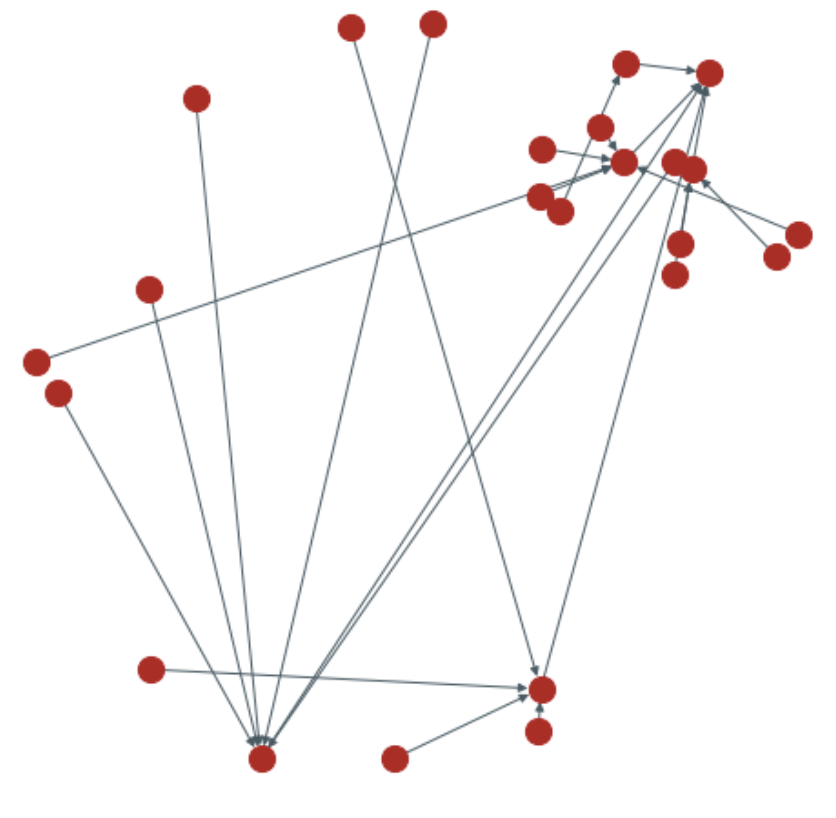
\includegraphics[width=\linewidth]{Immagini/comments-tree.png}
    \caption{Esempio di albero dei commenti.}
    \label{fig:comments-tree}
\end{figure}

\subsection{Grafo degli utenti}
\label{subsection:grafo_utenti}
Invece di considerare i commenti come argomenti, può essere considerato argomento ogni utente nella conversazione, andando a creare archi tra due utenti se un utente ha risposto almeno una volta ad un altro utente. Più formalmente costruire un grafo orientato $\mathcal{G = ⟨V, E⟩}$, dove i nodi $v \in \mathcal{V}$ sono utenti ed esiste un arco $(v_1,v_2) \in \mathcal{E}$ se l'utente $v_1$ ha risposto almeno una volta all'utente $v_2$.

In questo modo se ogni commento nell'albero della conversazione ha un utente univoco, l'Argumentation Framework risultante sarà comunque un albero, mentre se un utente risponde ad almeno due (o più) utenti il suo nodo nell'$AF$ avrà due (o più) archi uscenti, e se più commenti dello stesso utente vengono risposti da due (o più) utenti, il suo nodo nell'$AF$ avrà due (o più) archi entranti.

Estrarre delle semantiche da Argumentation Framework ricavati dal grafo degli utenti equivale ad estrarre gli utenti che soddisfano i requisiti delle varie semantiche.


\begin{figure}[h]
    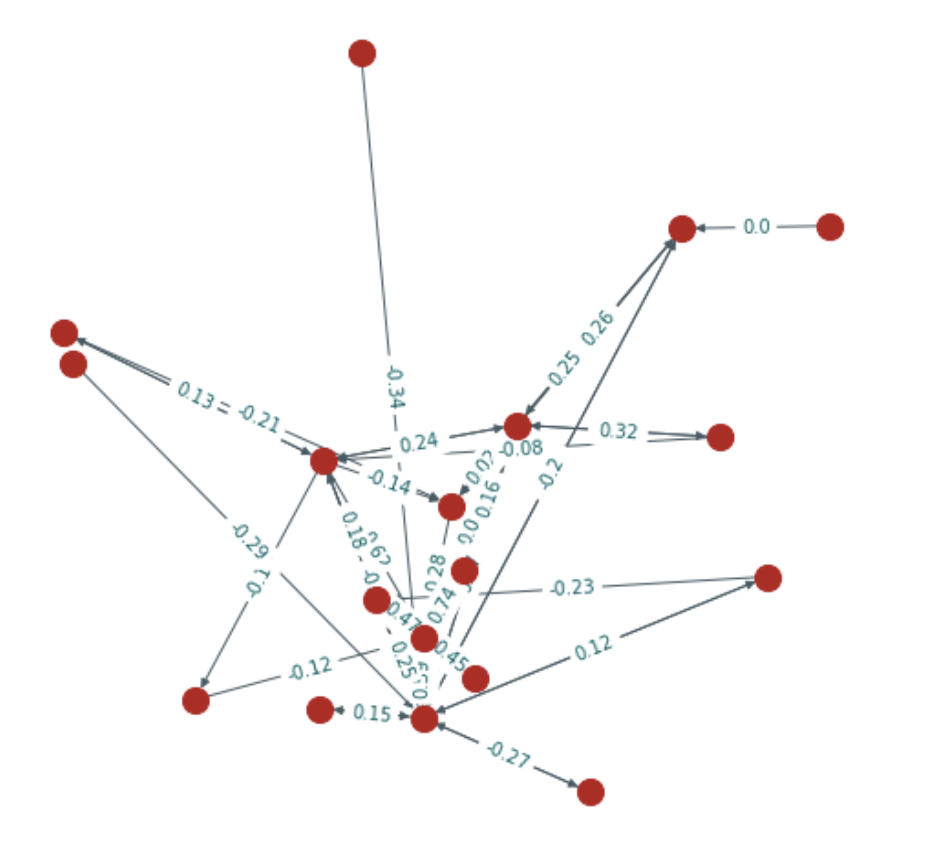
\includegraphics[width=\linewidth]{Immagini/users-graph.png}
    \caption{Esempio di grafo degli utenti.}
    \label{fig:users-graph}
\end{figure}

\subsection{Pesi delle relazioni}
\label{subsection:weight}
Le relazioni di risposta nell'albero dei commenti possono essere pesate in base alla combinazione di similarità e sentiment dei testi dei commenti.

\subsubsection{Similarity}
La \textit{similarity} è ricavata attraverso l'embedding dei testi dei commenti ricavati da un modello di Word2Vec pre-addestrato sulle news di Google \cite{googlenewsmodel}. Gli Word Embedding sono un insieme di tecniche per la rappresentazione vettoriale delle parole di un vocabolario, introdotti per la prima volta in \cite{mikolov2013distributed}, i quali sono capaci di catturare il contesto delle parole all'interno di un documento attraverso la \textit{distributional semantics}. I vettori risultanti codificano proprietà linguistiche nello spazio vettoriale e nella distanza tra di essi, ad esempio è possibile fare analogie come mostrato in figura \ref{fig:analogy}.

\begin{figure}
    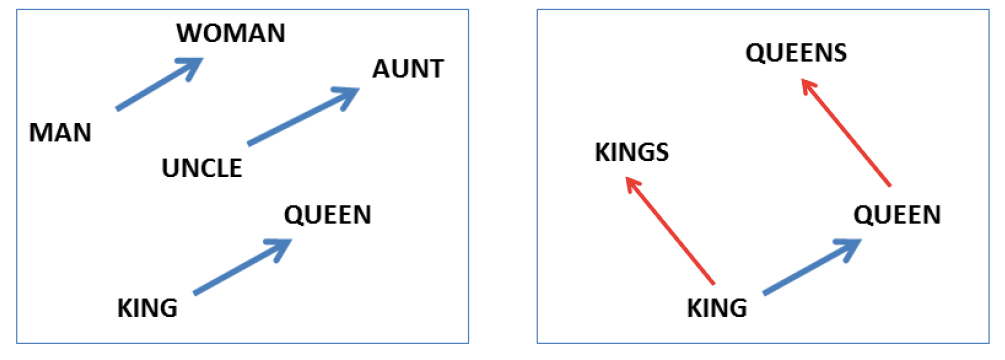
\includegraphics[width=\linewidth]{Immagini/king-queen.png}
    \caption{Analogie tra vettori.}
    \label{fig:analogy}
\end{figure}

L'emebedding dei testi dei commenti è ottenuto facendo la media degli embedding delle parole contenute. Infine la similarità tra due testi $c_1$ e $c_2$ si ricava con:

$$cosineSimilarity(c_1, c_2) = \frac{c_1 \cdot c_2}{||c_1|| ||c_2||}$$

che restituirà quindi un risultato compreso $\in [0, 1]$.

\subsubsection{Sentiment}
La \textit{sentiment analysis} si riferisce all'utilizzo dell'elaborazione del linguaggio naturale per identificare, estrarre e quantificare sistematicamente informazioni soggettive. L'analisi del sentiment è ampiamente applicata per analizzare social media per una varietà di applicazioni. Il valore è ricavato attraverso VADER \cite{hutto2014vader} uno strumento di analisi del sentiment basato su regole che è stato ideato specificamente per individuare la polarità nei testi espressi nei social media, ad esempio:

    $$sentiment(\ "\textbf{:)}" \ ) = 0.4588$$
    $$sentiment(\ "\textbf{:(}" \ ) = -0.4404$$

che restituirà quindi un risultato compreso $\in [-1, 1]$.

\subsubsection{Peso finale}
Il peso finale dell'arco è ottenuto prendendo in considerazione la similarità tra i commenti, in modo da da dare un valore maggiore a commenti simili e minore a commenti con similarità bassa, ed il sentiment. Se la polarità dei sentiment dei due commenti è la stessa allora è possibile dedurre che i commenti sono in accordo tra loro. Più precisamente:

$$weight = similarity_{c_1 c_2} \cdot sentiment_{c_1} \cdot sentiment_{c_2}$$

che restituirà quindi un risultato compreso $\in [-1, 1]$.

Dal segno del peso finale è possibile dedurre il tipo di relazione per Bipolar AF e per Bipolar Weighted AF. Sarà creata una relazione di \textbf{supporto} se il segno è positivo, di \textbf{attacco} altrimenti. 

\section{Analisi dei Social Media}
\label{section:data_sources}

\subsection {Twitter} %%%%%%%%%%%%%%%%%%%%%%%%%%%%%%%%%%%%%%%%%%%

Lo scraping del sito Web è vietato dal Twitter Terms of Service, quindi l'estrazione della conversazione avviene tramite API. Per accedere alla piattaforma delle API di twitter è necessario creare un Twitter developer account ed in seguito creare dal portale una applicazione nella quale si dichiara lo scopo dello dell'accesso ai contenuti e si richiedono i relativi permessi. Una volta ottenuta l'approvazione, vengono rilasciati delle credenziali per l'autenticazione agli endpoint. Gli step necessari sono:
  

\begin{itemize}  
    \item Andare su {\color{blue}\underline{\href{https://.dev.twitter.com}{Twitter Developers Site}}}
    \item Login con account di Twitter
    \item Andare su "My Applications"
    \item Creare una nuova applicazione
    \item Compilare con i dati richiesti
    \item Creare l'Access Token
    \item Scegliere il tipo di permessi
    \item Prendere nota delle impostazioni OAuth
    \item Infine, tutto il necessario per l'estrazione della conversazione è: \begin{itemize}
        \item Consumer key
        \item Consumer secret
        \item Access token
        \item Access token secret
    \end{itemize}
\end{itemize}

I contenuti messi a disposizione sono i Tweet pubblici, reperiti cercando parole chiave specifiche attraverso le Search API o chiedendo esempi di Tweet a determinati account attraverso le User API. Inoltre è possibile richiedere tweet specifici conoscendone l'id.

Al momento non è disponibile l'accesso alle conversazioni, la richiesta di tweet tramite le Search API o le User API restituisce solo un sottoinsieme dei tweet ed inoltre c'è un limite al numero di richieste giornaliere. Questo rende difficile cercare di ricostruire le conversazioni dai tweet restituiti dalla query. 

\subsubsection{Ricostruire la conversazione}
\label{ricostruire-conv}
La richiesta ad un determinato topic restituisce un campione di massimo 1000 tweet recenti.
Fra gli attributi presenti nei tweet è presente il campo \textbf{"in reply to status id"} che, se presente, contiene l'id del tweet al quale il tweet corrente sta rispondendo. Questo id può essere utilizzato per cercare di ricostruire la conversazione, facendo una richiesta tramite API per avere il tweet risposto e, se questo a sua volta risponde ad un altro tweet, continuare a seguire la catena di risposte (la conversazione). Per qualsiasi tweet con questo campo, possiamo:
\begin{itemize}
    \item trovare il tweet a cui quello corrente sta rispondendo, quindi ripetere la procedura per ogni tweet con questo attributo avvalorato in modo da ottenere delle sequenze di tweet.
    \item Una volta create le sequenze di tweet, se queste contengono elementi in comune, unire le sequenze creando un grafo della conversazione.
    \item Valutare la bontà della conversazione ottenuta mediante euristiche come ad esempio il numero di nodi (tweet) nel grafo della conversazione, la presenza di diramazioni o il numero di utenti distinti, in modo da poter scegliere la conversazione "migliore".
\end{itemize}

Quindi costruire grafo orientato e pesato della conversazione $\mathcal{G = ⟨V, E⟩}$, dove i nodi $v \in \mathcal{V}$ sono tweet ed esiste un arco $(v_1,v_2) \in \mathcal{E}$ se l'attributo \textbf{"in reply to status id"} di $v_1$ contiene l'id di $v_2$, pesato come descritto in \ref{subsection:weight}.

Tuttavia le API forniscono l'accesso solo ad un campione dei tweet, quindi potrebbe non essere possibile recuperare dei tweet quando si tenta di ricostruire la conversazione. Un'altra limitazione proviene dal numero di tweet iniziale che è possibile ottenere in risposta alla query, che risulta essere massimo 1000, dai quali è necessario filtrare i tweet che non contengono il campo \textbf{"in reply to status id"} avvalorato(di solito circa il 80\%). Inoltre i risultati ottenuti cambiano in modo notevole al variare della query e del momento in cui viene effettuata la richiesta. La maggior parte delle volte le conversazioni risultano essere sequenze lineari di nodi, ovvero grafi con archi in entrata $\leq 1$ ed archi in uscita $\leq 1$ come rappresentato in figura \ref{fig:comment-twitter}.

\begin{figure}[ht]
    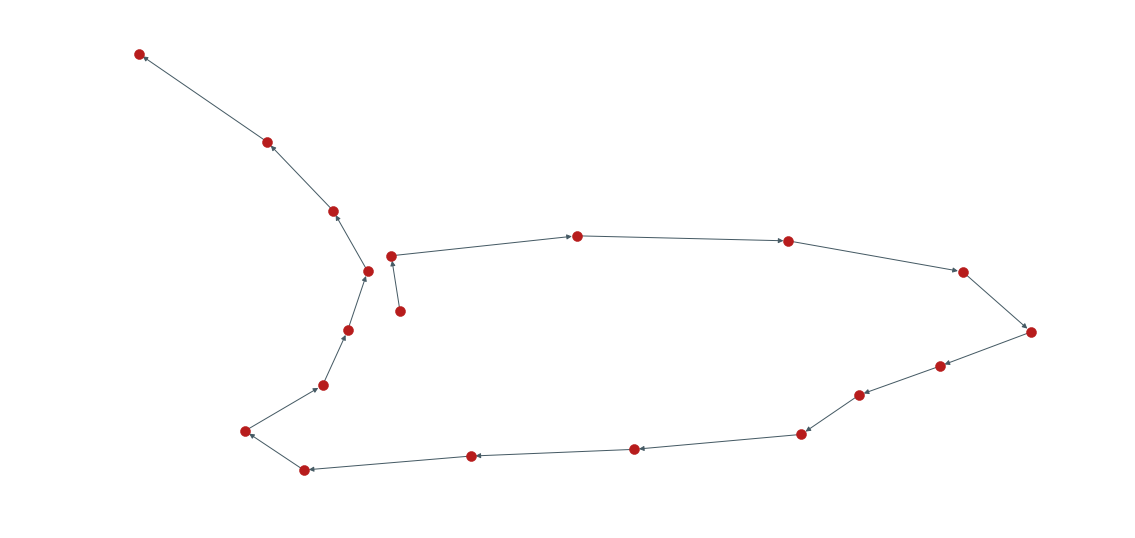
\includegraphics[width=\linewidth]{Immagini/twitter.png}
    \caption{Rappresentazione del grafo della conversazione, utilizzando come nodi i commenti.}
    \label{fig:comment-twitter}
\end{figure}

\subsubsection {Utenti come nodi}
Un altro approccio è quello descritto in sezione \ref{subsection:grafo_utenti}, ma con la differenza che qui non c'è l'albero della conversazione ma ci sono i 1000 tweet restituiti dalla richiesta API più eventuali altri tweet ottenuti seguendo il campo \textbf{"in reply to status id"}. Quindi viene costruito il grafo orientato pesato $\mathcal{G = ⟨V, E⟩}$, dove i nodi $v \in \mathcal{V}$ sono utenti ed esiste un arco $(v_1,v_2) \in \mathcal{E}$ se esiste almeno un tweet con utente $v_1$ e con l'attributo \textbf{"in reply to status id"} contenente l'id di un tweet appartenente all'utente $v_2$, pesato come descritto in \ref{subsection:weight}.

Anche qui si ripropongono i problemi presentati nella sezione precedente \ref{ricostruire-conv}, tuttavia il grafo risultante presenta nodi con archi in entrata $\geq 1$ ed archi in uscita $\geq 1$, come rappresentato in figura \ref{fig:users-twitter}.

\begin{figure}[H]
    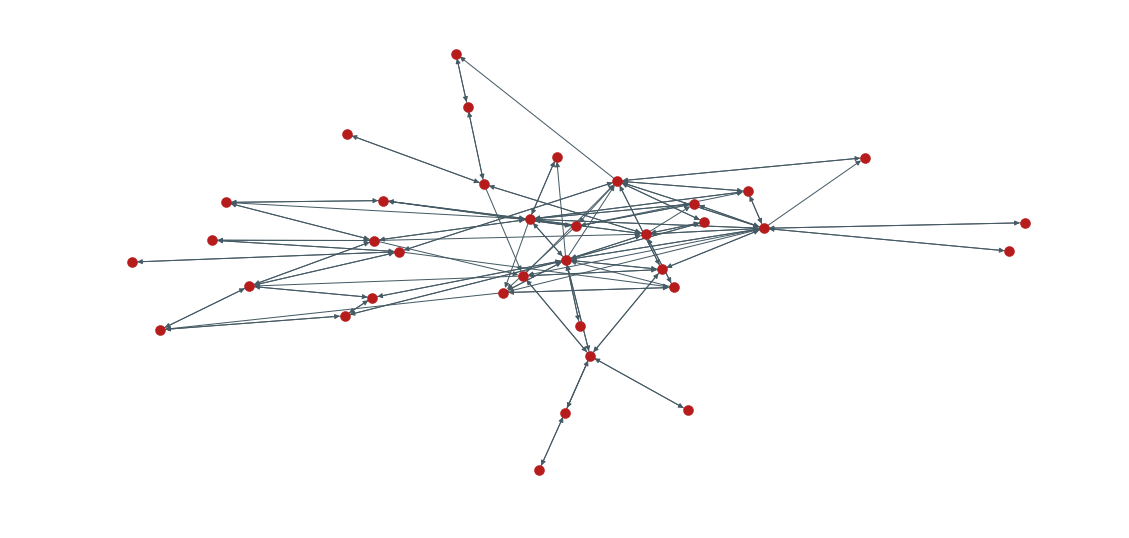
\includegraphics[width=\linewidth]{Immagini/twitter-users.png}
    \caption{Rappresentazione del grafo della conversazione, utilizzando come nodi gli utenti.}
    \label{fig:users-twitter}
\end{figure}



%%%%%%%%%%%%%%%%%%%%%%%%%%%%%%%%%%%%%%%%%%%%%%%%%%%%%%%%%%%%%%%
%%%%%%%%%%%%%%%%%%%%%%%%%%%%%%%%%%%%%%%%%%%%%%%%%%%%%%%%%%%%%%%
%%%%%%%%%%%%%%%%%%%%%%%%%%%%%%%%%%%%%%%%%%%%%%%%%%%%%%%%%%%%%%%
%%%%%%%%%%%%%%%%%%%%%%%%%%%%%%%%%%%%%%%%%%%%%%%%%%%%%%%%%%%%%%%
%%%%%%%%%%%%%%%%%%%%%%%%%%%%%%%%%%%%%%%%%%%%%%%%%%%%%%%%%%%%%%%


\subsection {Stackoverflow} %%%%%%%%%%%%%%%%%%%%%%%%%%%%%%%%%%%%%%%%%%%
Attraverso la libreria Stack API \cite{stackapi} è possibile fare richieste, tramite pyhton, alle API di Stackoverflow senza necessità di registrarsi.

\subsubsection {API}

\begin{lstlisting}[language=Python, caption=Stack API in Python]
site = StackAPI('stackoverflow')

# Richiedere una specifica domanda
site.fetch(
    'questions/<q_id>', 
    order='desc', 
    sort='votes', 
    filter='withbody')
    
# Richiedere tutte le risposte ad una domanda
site.fetch(
    'questions/<q_id>/answers', 
    order='desc', 
    sort='votes', 
    filter='withbody')

#  Richiedere tutti commenti ad una risposta   
site.fetch(
    'answers/<a_id>/comments', 
    order='desc', 
    sort='votes', 
    filter='withbody')
\end{lstlisting}

Di seguito è riportato un esempio per utilizzare le Stack API. Per prima cosa bisogna creare un oggetto StackAPI con il dominio di riferimento, in questo caso stackoverflow. Una volta creato è possibile:

\begin{itemize}
    \item Richiedere una specifica domanda, conoscendone l'id (reperibile dall'URL)
    \item Richiedere tutte le risposte ad una domanda, conoscendo l'id della domanda
    \item Richiedere tutti commenti ad una risposta, conoscendone l'id
\end{itemize}

\subsubsection {Commenti}

Per costruire l 'albero dei commenti è necessario:

\begin{itemize}
    \item \textbf{Nodo radice}: scegliere una domanda da cui costruire il nodo radice
    \item \textbf{Primo livello}: richiedere tutte le risposte a quella domanda
    \item \textbf{Secondo livello}: richiedere tutti commenti ad ogni risposta
\end{itemize}

Stackoverflow permette di costruire un albero con profondità massima di 3 livelli, in quanto ogni domanda può avere delle risposte e queste possono avere dei commenti.
 

\subsubsection {Utenti}
Per costruire il grafo degli utenti è necessario:

\begin{itemize}
    \item \textbf{Costruire l'albero dei commenti}: tramite il procedimento descritto nella sezione precedente
    \item \textbf{Unire i nodi}: unire i nodi che hanno lo stesso utente
\end{itemize}

Nelle domande analizzate è capitato raramente di riuscire ad unire nodi nell'albero dei commenti, raramente un utente fornisce più risposte alla stessa domanda. Può capitare invece che lo stesso utente fornisca più commenti. 


%%%%%%%%%%%%%%%%%%%%%%%%%%%%%%%%%%%%%%%%%%%%%%%%%%%%%%%%%%%%%%%
%%%%%%%%%%%%%%%%%%%%%%%%%%%%%%%%%%%%%%%%%%%%%%%%%%%%%%%%%%%%%%%
%%%%%%%%%%%%%%%%%%%%%%%%%%%%%%%%%%%%%%%%%%%%%%%%%%%%%%%%%%%%%%%
%%%%%%%%%%%%%%%%%%%%%%%%%%%%%%%%%%%%%%%%%%%%%%%%%%%%%%%%%%%%%%%
%%%%%%%%%%%%%%%%%%%%%%%%%%%%%%%%%%%%%%%%%%%%%%%%%%%%%%%%%%%%%%%

\subsection {Reddit} %%%%%%%%%%%%%%%%%%%%%%%%%%%%%%%%%%%%%%%%%%%

Attraverso la libreria PRAW \cite{praw} è possibile fare richieste, tramite pyhton, alle API di Reddit. Necessario registrarsi per ricevere il \textbf{CLIENT ID} ed il \textbf{CLIENT SECRET}. i passi da seguire sono:

\begin{itemize}
    \item \textbf{Reddit Account}:	creare un account all'indirizzo reddit.com.
    \item \textbf{Client ID e Client Secret}: seguendo le istruzioni riportate in \url{https://github.com/reddit-archive/reddit/wiki/OAuth2-Quick-Start-Example#first-steps}
    \item \textbf{User Agent}:	Creare un user agent univoco in modo da permettere Reddit a determinare la fonte delle richieste.
\end{itemize}

\subsubsection {API}

\begin{lstlisting}[language=Python, caption=Stack API in Python]
reddit = praw.Reddit(
    client_id='XXXXXXXXXXXXXX',
    client_secret='XXXXXXXXXXXXXXXXXXXXXXXXXXX',
    user_agent=' 'linux:com.example.argumentation:v0.0.1 (by /u/anzianotti)'
)

# Richiedere una specifica domanda
reddit.submission(submissionId)

# Esapndere i risultati inizialmente restituiti
submission.comments.replace_more(limit=None)

# Prendere i commenti
comments = submission.comments
    
    
\end{lstlisting}

Di seguito è riportato un esempio per utilizzare le API di reddit tramite PRAW. Per prima cosa bisogna creare un oggetto reddit con il \textbf{client id}, il \textbf{client secret} e l'\textbf{user agent}, in questo caso stackoverflow. Una volta creato è possibile:

\begin{itemize}
    \item Richiedere una specifica submission, conoscendone l'id (reperibile dall'URL)
    \item Espandere i risultati facendo restituire anche i commenti nascosti oltre un certo livello (da browser sono i commenti disponibili cliccando sul tasto "view more comments")
    \item Recuperare la lista degli oggetti commento
\end{itemize}

\subsubsection {Commenti}
Per costruire l 'albero dei commenti è necessario:

\begin{itemize}
    \item \textbf{Nodo radice}: scegliere la submission contenente la domanda da cui costruire il nodo radice
    \item \textbf{Esplorare la submission}: Esplorare la submission costruendo l'albero
\end{itemize}

Reddit non pone limiti alla profondità dei commenti, di conseguenza l'albero non ha dimensioni prefissate.

\begin{figure}
    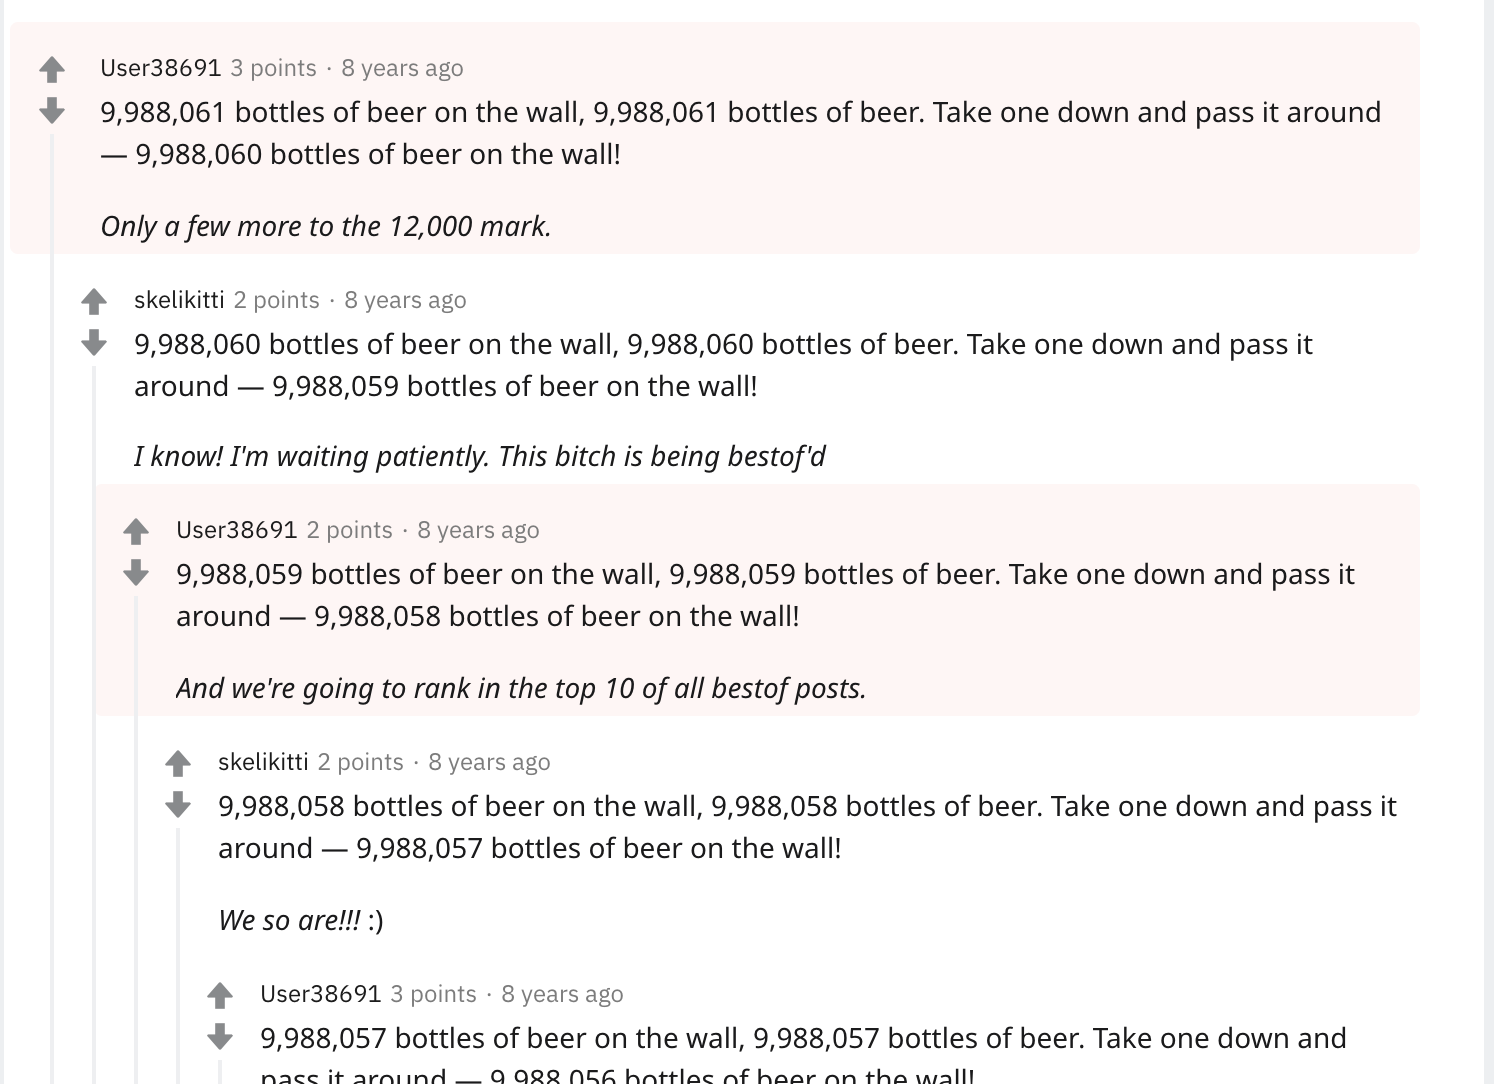
\includegraphics[width=\linewidth]{Immagini/reddit-comment-nesting.png}
    \caption{Esempio di reddit submission per trovare la profondità massima dei commenti.}
    \label{fig:reddit-comment-nesting}
\end{figure}


\subsubsection {Utenti}

Per costruire il grafo degli utenti è necessario:

\begin{itemize}
    \item \textbf{Costruire l'albero dei commenti}: tramite il procedimento descritto nella sezione precedente
    \item \textbf{Unire i nodi}: unire i nodi che hanno lo stesso utente
\end{itemize}

Il risultato dipende dalla submission in analisi, ma le conversazioni molto polarizzate invogliano gli utenti a commentare più volte, andando ad unire più nodi nell'albero dei commenti.


% Fatti generati argument/1, attac- k/2, support/2, rel_weight/3

% descrizione vader e altri componenti utilizzati

